\chapter{Files}
	\label{ch:files}

	This chapter explains:
	\begin{itemize}
    \item what a text file is;
    \item how to read and write data to files;
    \item how to manipulate folder paths and names.
	\end{itemize}

	\section{Introduction}
		You have already made use of files, in the sense of having used the IDE to create files containing VB programs, and having used Windows to view a hierarchical structure of folders (directories). In this chapter, we will look at the nature of the information you may choose to store in files, and how you can write programs to manipulate files.
		
		Initially, let us clarify the difference between RAM (random-access memory) and file storage devices (e.g. USB thumb drives, hard disk drives, SSDs and DVDs). Storage capacity is measured in bytes in all these cases. There are several major differences between RAM and file storage:
		\begin{itemize}
      \item RAM is used to store programs as they execute. They are copied from a file storage device immediately before execution.
      \item The time to access an item in RAM is much faster.
      \item The cost of RAM is higher (megabyte for megabyte).
      \item Data in RAM is temporary: it is erased when power is switched off. File storage devices can hold data permanently.
		\end{itemize}
		The capacity of file storage devices is higher. CD-ROMs used to have a capacity of around 740 Mbyte (megabytes), DVD (Digital Versatile Disks) have a capacity of up to 15 Gbyte (gigabyte, 1024 Mbyte) and BluRay discs up to 100 Gbyte. CD-ROMs, DVDs and BluRay (BD) have writeable and re-writeable versions. Typical hard drives (HDD) can hold around several terabyte, the same goes for solid state drives (SSD) and USB memory sticks or SD cards can hold up to 1 Tbyte. However, technology is evolving rapidly – the race is to create ever cheaper, smaller storage devices that modern computer software requires, especially in the area of high-quality video and images.


	\section{The essentials of streams}
		Streams let us access a file as a sequence of items. The term 'stream' is used, in the sense of a stream of data flowing in or out of the program. Let us introduce the jargon, which is similar in most programming languages. If we wish to process the data in an existing file, we must:
		\begin{enumerate}
			\item	Open the file.
			\item	Read (input) the data item-by-item into variables.
			\item	Close the file when we have finished with it. 
		\end{enumerate}
		To transfer some data from variables into a file, we must:
		\begin{enumerate}
			\item	Open the file.
			\item	Output (write) our items in the required sequence.
			\item	Close the file when we have finished with it.
		\end{enumerate}
		
		Note that, when reading from a file, all we can do is read the next item in the file. If for example, we only needed to examine the last item in a file, we would have to code a loop to read each preceding item in turn, until the required item is reached. For many tasks, it is convenient to visualize a text file as a series of lines, each made up of a number of characters. Each line is terminated by an end-of-line marker, consisting of either the line-feed character, or the carriage-return character, or both of these. Your response to this might be to say 'I just hit Enter at the end of a line!'. Behind the scenes, Windows software will put a line-feed character and a carriage-return character at the end of each line. Most of this intricacy is hidden by VB.
		
		As well as files containing lines of text, VB can also manipulate files containing binary data, such as images. However, such data is usually arranged in a more complicated format within files.
		
		We shall make use of the VB classes that allow us to access a file line-by-line, as text strings. This is particularly useful, because many applications (such as word-processors, text editors and spreadsheets) can read and write such files.


	\section{The \keyword{StreamReader} and \keyword{StreamWriter} classes}
		To read and write lines of text, we will use:
		\begin{itemize}
			\item The \keyword{ReadLine} method of \keyword{StreamReader}. This reads a whole line of text into a string, excluding the end-of-line marker. (If we need to split the line into separate parts, we can use the \keyword{Split} function described in \Cref{ch:strings}.)
			\item The \keyword{StreamWriter} class. This has two main methods: \keyword{Write} and \keyword{WriteLine}. They both write a string to a file, but \keyword{WriteLine} adds the end-of-line marker after the string. We can also use \keyword{WriteLine} with no string argument, where an end-of-line marker is written to the file.
			\item The \keyword{OpenText} and \keyword{CreateText} methods of the \keyword{File} class. These are shared methods, and provide us with a new instance of a text stream. A selection of other methods and properties of the \keyword{File} class is covered later in this chapter.
		 \end{itemize}
		 The file classes are in the \keyword{System.IO} namespace. This is not automatically imported, so we must put:
		\begin{lstlisting}
Imports System.IO
		\end{lstlisting}
		at the very top of all our file-processing programs.


	\section{File output}
		The File Output program opens a file and writes three lines to it. The user interface only consists of a single button, so is not shown. Here is the code:
		\begin{lstlisting}
Private Sub Button1_Click(
		sender As System.Object,
		e As System.EventArgs)
		Handles Button1.Click
	' write some lines of text to the file
	Dim outputStream As StreamWriter =
			File.CreateText("c:\myfile.txt")
	outputStream.WriteLine("This file will")
	outputStream.WriteLine("contain 3")
	outputStream.WriteLine("lines of text.")
	outputStream.Close()
End Sub
		\end{lstlisting}
		First we create and open the file:
		\begin{lstlisting}
Dim outputStream As StreamWriter =
	File.CreatText("c:\myfile.txt")
		\end{lstlisting}
		Here, we make use of the shared method \keyword{CreateText} from the \keyword{File} class. This creates a new \keyword{StreamReader} object for us, and opens the file. Note that there are two items which refer to the file:
		\begin{itemize}
			\item There is a string which specifies the file name that the operating system uses when it displays folders: \keyword{"c:\textbackslash myfile.txt"}. Alter this path if you wish to create the file in a different place. If you omit the folder name and just use \keyword{myfile.txt}, then the file will be created in a folder named \keyword{bin}, which is a sub-folder of your current VB project.
			\item There is a variable which we chose to name as \keyword{outputStream}. It is an instance of the class \keyword{StreamWriter}, which provides us with the \keyword{WriteLine} method. The use of \keyword{CreateText} associates \keyword{outputStream} with the file \keyword{"c:\textbackslash myfile.txt"}.
		\end{itemize}
		To actually write a line of text to the file, we use \keyword{WriteLine}, as in:
		\begin{lstlisting}
outputStream.WriteLine("This file will")
		\end{lstlisting}
		If the data we wish to place in the file is typed in by the user – perhaps in a text box – we would put:
		\begin{lstlisting}
outputStream.WriteLine(TextBox1.Text)
		\end{lstlisting}
		If the file existed already, its original contents will be erased, and replaced by the three lines.
		
		Finally, we close the file:
		\begin{lstlisting}
outputStream.Close()
		\end{lstlisting}
		This ensures that any data in transit is actually placed in the file, and also allows the file to be reopened for reading or writing.

		In summary, our file output process was:
		\begin{itemize}
      \item to open the file \keyword{"c:\textbackslash myfile.txt"};
      \item to output (write) some strings to the file;
      \item to close the file.
		\end{itemize}


		\begin{stqb}
			\begin{STQ}
				\item	Explain what the following code does:
					\begin{lstlisting}
Dim lines, stars As Integer
Dim fileName As String = "c:\pattern.txt"
Dim streamOut As StreamWriter =
		File.CreateText(fileName)
For lines = 1 To 10
		For stars = 1 To lines
			streamOut.Write("*")
		Next
		streamOut.WriteLine()
Next
streamOut.Close()
					\end{lstlisting}
			\end{STQ}
		\end{stqb}

	\section{File input}
		Here we examine the program named File Input, which opens a file, inputs its contents and displays it in a text box. The program makes use of \keyword{NewLine} when placing a string in the text box. This requires an additional import, so the first two lines of the program are:
		\begin{lstlisting}
Imports System.IO
Imports Microsoft.VisualBasic.ControlChars
		\end{lstlisting}
		\begin{figure}[tbh]
			\centering
			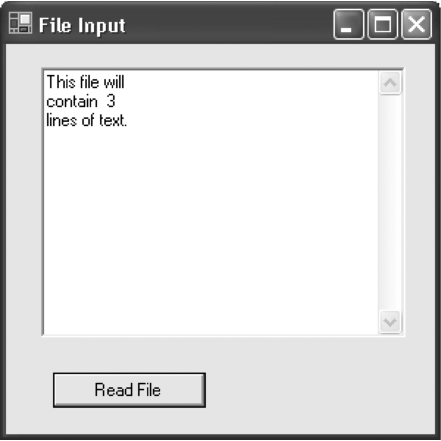
\includegraphics[width=7cm]{files_input_screen}
			\caption{Screenshot of the File Input program.}
			\label{fig:files_input_screen}
		\end{figure}
		The screenshot (taken after the button was clicked) is given in \Vref{fig:files_input_screen}. Here is the code:
		\begin{lstlisting}
Private Sub Button1_Click(
		sender As System.Object,
		e As System.EventArgs)
		Handles Button1.Click
	'read the file line-by-line
	Dim inputStream As StreamReader =
			File.OpenText("c:\myfile.txt")
	Dim line As String
	line = inputStream.ReadLine()
	While line <> Nothing
		TextBox1.AppendText(line & NewLine)
		line = inputStream.ReadLine()
	End While
	inputStream.Close()
End Sub
		\end{lstlisting}
		The code is contained in the method \keyword{Button1\_Click}. The file we choose to input is the one that was created by the previous File Output program, containing three lines of text.

		First, we create a stream to access the file:
		\begin{lstlisting}
Dim inputStream As StreamReader =
	File.OpenText("c:\myfile.txt")
		\end{lstlisting}
		(If the file we specify cannot be found, an exception will be produced. For now, we ignore this possibility, but discuss it later in this chapter.)

		Then we use \keyword{ReadLine} to input the series of lines in the file, appending each one to our text box. There is one crucial point here: we don't know how many lines are in the file, so we set up a loop which terminates when there is nothing more to read:
		\begin{lstlisting}
line = inputStream.ReadLine()
While line <> Nothing
	TextBox1.AppendText(line & NewLine)
	line = inputStream.ReadLine()
End While
		\end{lstlisting}
		When \keyword{ReadLine} runs out of lines to read, it returns Nothing, and this is assigned to line. Nothing is a keyword in VB, indicating that the object does not exist.
		
		Note that we have used \keyword{ReadLine} twice. The first \keyword{ReadLine} prior to the loop is needed so that the first time \keyword{While} tests line, it has a value.
		
		Each line is placed at the end of any existing text already in the text box, by using \keyword{Append}. Because \keyword{ReadLine} does not provide us with the end-of-line characters, we need to use \keyword{NewLine}. If we omitted this, the text box would contain one long line, with no breaks.
		
		Reading a file line-by-line allows us to process each line individually (as we do in the File Search program below). Alternatively, it might be more appropriate to read the whole file into one long string, complete with end-of-line markers. In this case, VB provides us with a method named \keyword{ReadToEnd}, which we use for the text editor program shown later.

		In summary, the program:
		\begin{enumerate}
			\item	opens a file;
			\item	inputs lines from the file and appends them to the text box, as long as the end of the file is not reached;
			\item	closes the file.
		\end{enumerate}


		\begin{stqb}*
			\begin{STQ}
				\item	The following code is meant to display the length of each line in a file. Explain any problems.
					\begin{lstlisting}
Dim fileName As String = "c:\tempvb7.txt"
Dim stream As StreamReader = File.OpenText(fileName)
Dim line As String
	
line = stream.ReadLine()
While line <> Nothing
		line = stream.ReadLine()
		TextBox1.AppendText("length: " & line.Length & ",")
End While
stream.Close()
					\end{lstlisting}
				\item	Explain any problems in this code:
					\begin{lstlisting}
Dim fileName As String = "c:\tempvb7.txt"
Dim stream As StreamReader = File.OpenText(fileName)
Dim line As String
line = stream.ReadLine()
While line <> Nothing
		TextBox1.AppendText(line)
End While
stream.Close()
					\end{lstlisting}
			\end{STQ}
		\end{stqb}


	\section{File searching}
		Searching a file for an item that meets some specified criteria is a classic task. Here we will construct a program which searches a file of exam marks, which takes the form:
		\begin{lstlisting}
J.Doe, 43, 67
D.Bell, 87, 99
M.Parr, 54, 32
J.Hendrix, 67, 43
etc...
		\end{lstlisting}
		We might create this file by writing and running a VB program, or with a text editor. Each line is split into three areas, separated by commas. However, we will allow for extra spaces. In data processing, such areas are known as fields. The program will allow us to enter a filename, and to enter a student name, which we assume is unique. If the names are not unique, we would have to introduce an extra field to hold a unique identification number for each person. The program will search the file, and display the marks for our chosen student. The code we need to add to our previous file input example is a \keyword{While} which terminates when the end of the file is encountered or when the required name is found. We will use the \keyword{Split} function to separate the three fields.
		
		Because there are two ways that the loop can terminate, we introduce an additional variable, \keyword{found}, to indicate whether the item was found or not. Note that we expect that the item will sometimes not be found – it is not regarded as an error, and we code this with \keyword{If} rather than using exceptions.

		The informal English structure of the search is:
		\begin{lstlisting}
found = False
While (more lines to read) And found = False
	read line
	split line into three fields
	If first field matches name Then
		found = True
		display rest of fields in labels
	End If
End While
If Not found
	display a warning
End If
		\end{lstlisting}
		\begin{figure}[tbh]
			\centering
			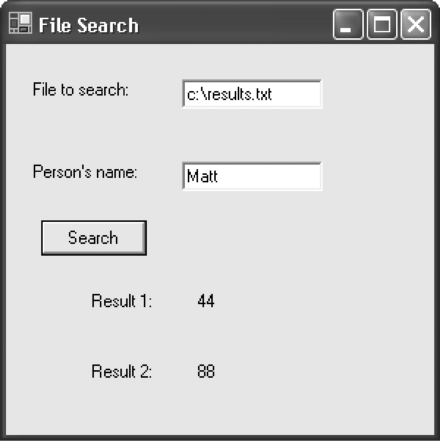
\includegraphics[width=7cm]{files_search_screen}
			\caption{Screenshot of File Search program.}
			\label{fig:files_search_screen}
		\end{figure}
		We have provided a search button, which causes the file to be opened and searched. The user can select any file for searching. \Vref{fig:files_search_screen} shows the screenshot, and here is the code.
		\begin{lstlisting}
Private Sub Button1_Click(
		sender As System.Object,
		e As System.EventArgs)
		Handles Button1.Click
	Dim line As String
	Dim words(3) As String	
	Dim found As Boolean = False
	Dim inputStream As StreamReader
	'clear any previous results
	Result1Box.Text = ""
	Result2Box.Text = ""
	If FileNameBox.Text = "" Then
		MessageBox.Show("Error: missing file name!")
	ElseIf StudentNameBox.Text = "" Then
		MessageBox.Show("Error: missing student name!")
	Else
		inputStream = File.OpenText(FileNameBox.Text)
		line = inputStream.ReadLine()
		While (line <> Nothing) And found = False
			words = Split(line, ",")
			If Trim(words(0)) = StudentNameBox.Text Then
				Result1Box.Text = Trim(words(1))
				Result2Box.Text = Trim(words(2))
				found = True
			Else
				line = inputStream.ReadLine()
			End If
		End While
		If Not found Then
			MessageBox.Show(StudentNameBox.Text & " not found")
		End If
		inputStream.Close()
	End If
End Sub
		\end{lstlisting}

		\begin{stqb}*
			\begin{STQ}
				\item Amend the search program so that the searching is done in a case-insensitive way (i.e. so that john matches john, John and JOHN).
				\item	Explain the problem that would arise if we re-coded our search loop with \keyword{Or}, as in:
		\begin{lstlisting}
While (line <> Nothing) Or found = False
		\end{lstlisting}
			\end{STQ}
		\end{stqb}


	\section{Files and exceptions}
	File input–output is a major source of exceptions. For example, the file name supplied by the user might be incorrect, the disk might be full, or the user might remove an SD card or USB thumb drive while reading is in progress. We can minimize the effects of incorrectly entered file names by using file dialogs (covered later), which let the user browse folders and click on file names, rather than typing the names into text boxes. But exceptions will still occur. In \Cref{ch:exceptions} we covered exceptions, and here we examine exceptions as they relate to files.
		
		A number of exceptions can be thrown when we access files. Here is a selection:
		\begin{itemize}
      \item The \keyword{.File.OpenText} method can throw a number of exceptions. We shall single out \keyword{FileNotFoundException} in particular.
      \item The \keyword{ReadLine} method of class \keyword{StreamReader} and the \keyword{WriteLine} method of class \keyword{StreamWriter} can throw an \keyword{IOException}, along with other classes of exceptions.
		\end{itemize}
		Here is another version of the search program, with exception-handling:
		\begin{lstlisting}
Private Sub Button2_Click(
		sender As System.Object,
		e As System.EventArgs)
		Handles Button2.Click
	'search the file – with exception-handling
	Dim line As String
	Dim words(3) As String
	Dim found As Boolean = False
	Dim inputStream As StreamReader
	'clear any previous results
	Result1Box.Text = ""
	Result2Box.Text = ""
	If FileNameBox.Text = "" Then
		MessageBox.Show("Error: missing file name!")
	ElseIf StudentNameBox.Text = "" Then
		MessageBox.Show("Error: missing student name!")
	Else
		Try
			inputStream = File.OpenText(FileNameBox.Text)
			line = inputStream.ReadLine()
			While (line <> Nothing) And found = False
				words = Split(line, ",")
				If Trim(words(0)) = StudentNameBox.Text Then
					Result1Box.Text = Trim(words(1))
					Result2Box.Text = Trim(words(2))
					found = True
				Else
					line = inputStream.ReadLine()
				End If
			End While
			If Not found Then
				MessageBox.Show(StudentNameBox.Text
						& " not found")
			End If
			inputStream.Close()
		Catch problem As FileNotFoundException
			MessageBox.Show("Error – file not found: "
						& FileNameBox.Text
						& ". Re-enter name.")
		Catch problem As Exception
			MessageBox.Show("Error concerning file: "
						& FileNameBox.Text
						& ". " & problem.message())
		End Try
	End If
End Sub
		\end{lstlisting}
		We have singled out \keyword{FileNotFoundException} as the most likely exception, and have produced a specific error message. Other exceptions might occur, but they cannot be neatly classified – so we choose to catch them all in one place, by referring to the class \keyword{Exception}.


	\section{Message boxes and dialogs}
		Sometimes we need to bring the user's attention to a vital decision or piece of information. Merely displaying some text in a label is not enough. VB provides a range of overloaded message box methods to provide configured dialogs. In addition, there are specific dialogs to request file names from the user, which we review later. Here are the message box methods:
		\begin{lstlisting}
MessageBox.Show(message)
MessageBox.Show(message, title)
MessageBox.Show(message, title, buttons)
MessageBox.Show(message, title, buttons, icon)
		\end{lstlisting}
		The arguments are as follows:
		\begin{itemize}
      \item the message is positioned in the centre of the message box;
      \item the title argument goes at the top of the message box;
      \item the buttons argument is a constant, specifying any buttons we need. For example we might require yes/no buttons;
      \item the icon argument specifies a symbol, such as a large exclamation mark or question mark.
		\end{itemize}
		The \keyword{Show} method also returns a code which we can examine to find out which button was clicked. There is a set of \keyword{DialogResult} constants which we can use for comparison. \Vref{fig:files_msgbox_screen1,fig:files_msgbox_screen2} show some examples, which show a warning message and a question.
		\begin{figure}[bth]
			\centering
			\begin{minipage}[t]{.45\textwidth}
			  \centering
				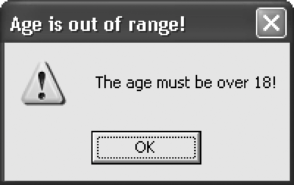
\includegraphics[width=5cm]{files_msgbox_screen1}
				\caption{Warning with a message box.}
				\label{fig:files_msgbox_screen1}
			\end{minipage}\hfill% create void between figures
			\begin{minipage}[t]{.45\textwidth}
				\centering
				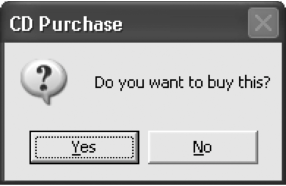
\includegraphics[width=5cm]{files_msgbox_screen2}	
				\caption{Question with a message box.}
				\label{fig:files_msgbox_screen2}
			\end{minipage}
		\end{figure}
		
		Here is the code. Note the style of calling the function method within an \keyword{If}, which accomplishes the dual role of displaying the message box and testing the result. When you run the code, you will see that the user cannot return to the form which displayed the message. First, the message box must be closed one way or another. The message box is described as \emph{modal}.
		\begin{lstlisting}
'warning
MessageBox.Show("The age must be over 18!",
			"Age is out of range!",
			MessageBoxButtons.OK,
			MessageBoxIcon.Exclamation)
'question
If MessageBox.Show("Do you want to buy this?",
			"CD Purchase",
			MessageBoxButtons.YesNo,
			MessageBoxIcon.Question)
		= DialogResult.Yes Then
	MessageBox.Show("user clicked Yes")
Else
	MessageBox.Show("user clicked No")
End If
		\end{lstlisting}


		\begin{stqb}
			\begin{STQ}
				\item Write code to display a message box which asks the question
					\begin{quote}
Is Paris the capital of France?
					\end{quote}
					Display suitable responses to the user's replies.
			\end{STQ}
		\end{stqb}


	\section{Using file dialogs}
		When a user needs to open a file using a word-processor or editor, they will make use of a file dialog window, which allows them to browse directories and to click on a selected file. Often, an application makes this available via a drop-down file menu at the top left of a window.
		\begin{figure}[tbh]
			\centering
			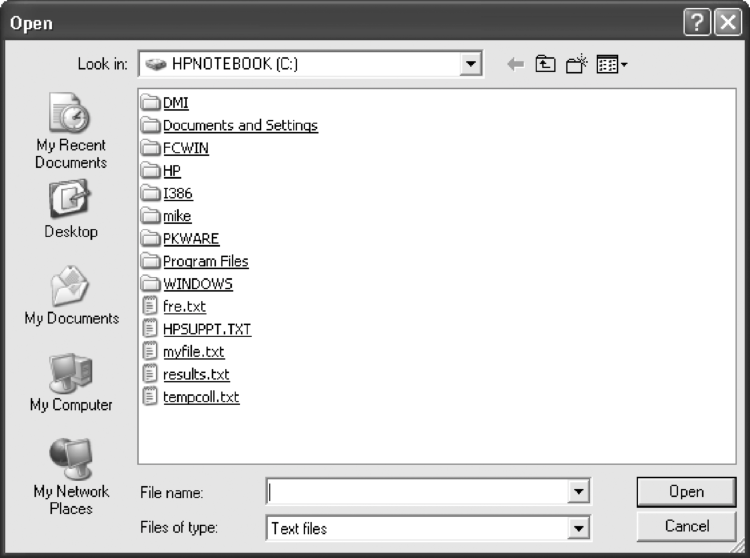
\includegraphics[width=11cm]{files_OpenFileDialog_screen}
			\caption{And \keyword{OpenFileDialog} in action.}
			\label{fig:files_OpenFileDialog_screen}
		\end{figure}
		
		In VB, we are provided with the \keyword{OpenFileDialog} and \keyword{SaveFileDialog} classes. \Vref{fig:files_OpenFileDialog_screen} shows the appearance of an open dialog. The steps to follow when programming the file dialogs are:
		\begin{itemize}
			\item We select the dialog from the \ui{Dialogs} section of the toolbox, and place it on the form. It moves to the component tray, because it does not reside on the form. The first dialog we create will be named \keyword{OpenFileDialog}1.
      \item We set its properties as required – at design-time if we know them. One of the most useful properties is its \keyword{InitialDirectory}, which is a string containing a directory path.
			\item We display the dialog using its \keyword{ShowDialog} method, which also returns a result to the program. The result indicates how the user closed the dialog, e.g. by clicking the \ui{Open} or the \ui{Cancel} button. The \keyword{DialogResult} class contains a list of conveniently named constants we can use.
      \item We make use of the \keyword{FileName} property, which provides us with a string containing the name of the selected file.
		\end{itemize}
		Here is some VB code which creates an \keyword{OpenFileDialog}:
		\begin{lstlisting}
If SaveFileDialog1.ShowDialog() = DialogResult.OK Then
	MessageBox.Show(OpenFileDialog1.FileName)
End If
		\end{lstlisting}
		We set its \keyword{InitialDirectory} property to the \keyword{c:\textbackslash} directory.
		
		We then use \keyword{ShowDialog} in an \keyword{If} statement. This compares the number returned from \keyword{ShowDialog} to the constant \keyword{DialogResult.OK}. (Using constants provided by VB is less error-prone than using the numbers themselves.) In this context, 'OK' means that the 'Open' button was clicked. If the user closed the dialog by shutting it down or by cancelling, we take no action. The process of using a \keyword{SaveFileDialog} is virtually identical. The following text editor program shows the dialogs incorporated with a menu containing 'Save', 'Open', and 'Save As' options.
		
		When you have understood the operation of file dialogs, it is recommended that you use them rather than using a text box for file name input. They are slightly more difficult to program, but are much more resistant to file name errors.


	\section{Creating a menu}
		Many applications provide a vast range of facilities, with the consequence that allocating a button to initiate each facility is impractical: too much valuable screen space would be consumed. The menu is one solution to the space problem. It occupies very little space, and its options only become visible when the menu is clicked.
		
		In VB, we can create a menu at the top of a form by selecting \ui{MenuStrip} from the \ui{Menus \& Toolbars} section of the toolbox and placing it on a form. (VB then opens the \ui{component} tray, and places the menu there). Initially we are asked if the menu is to be a \ui{MenuItem}, a \ui{ComboBox}, or a \ui{TextBox}. Choose \ui{MenuItem}. Once this is done, some 'Type Here' prompts appear, as in \Vref{fig:files_menu}. These allow us to set the text that appears on the menus.
	 	\begin{itemize}
      \item We can create a new menu item by typing underneath the existing menu, or
      \item We can create a heading for a new list of menu items by typing at the right of the existing menu name.
		\end{itemize}
		\begin{figure}[tbh]
			\centering
			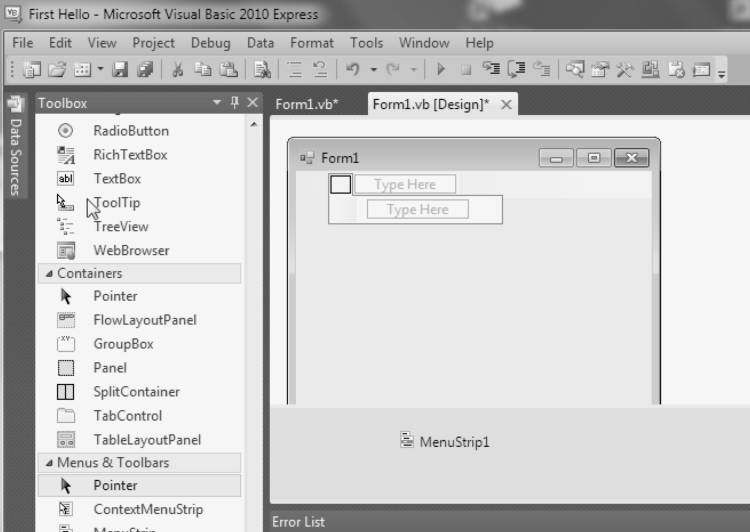
\includegraphics[width=12cm]{files_menu}
			\caption{Creating a menu at design-time.}
			\label{fig:files_menu}
		\end{figure}

		We have created a menu named 'File', and have added the items 'Open . . .', 'Save', 'Save As . . .' and 'Exit'. There is a Windows convention of using a file menu at the left of the form, and of using '. . .' to indicate that further choices will appear. When a menu item has been created, we can change its name at design-time by clicking on it with the right mouse button, and selecting its name via the properties window. 
		
		Here is the code for a program named Text Editor, and the screenshot is shown in \Vref{fig:files_text_editor_screen}.
		\begin{figure}[tbh]
			\centering
			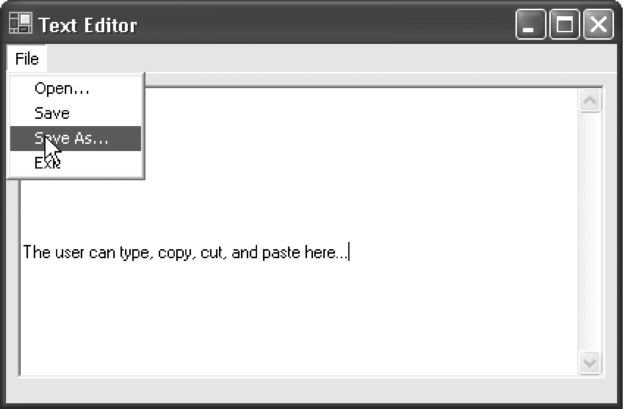
\includegraphics[width=10cm]{files_text_editor_screen}
			\caption{Screenshot of the text editor program.}
			\label{fig:files_text_editor_screen}
		\end{figure}


		
		We renamed the menu items to \keyword{OpenMenu}, \keyword{SaveMenu}, \keyword{SaveAsMenu} and \keyword{ExitMenu}. VB creates event-handling methods based on these names.
		\begin{lstlisting}
Private currentFile As String = "" 'instance variable
Private Sub OpenToolStripMenuItem_Click(sender As System.Object,
			e As System.EventArgs)
			Handles OpenToolStripMenuItem.Click
	Dim inputStream As StreamReader
	OpenFileDialog1.InitialDirectory = "c:\"
	If OpenFileDialog1.ShowDialog() =
			DialogResult.OK Then
		currentFile = OpenFileDialog1.FileName
		inputStream = File.OpenText(currentFile)
		TextBox1.Text = inputStream.ReadToEnd()
		inputStream.Close()
	End If
End Sub
Private Sub SaveToolStripMenuItem_Click(sender As System.Object,
			e As System.EventArgs)
			Handles SaveToolStripMenuItem.
Click
	If currentFile <> "" Then
		Dim outputStream As StreamWriter =
			File.CreateText(currentFile)
		outputStream.Write(TextBox1.Text)
		outputStream.Close()
	End If
End Sub
Private Sub SaveAsToolStripMenuItem_Click(sender As System.Object,
			e As System.EventArgs)
			Handles SaveAsToolStripMenuItem.Click
	Dim outputStream As StreamWriter
	SaveFileDialog1.InitialDirectory = "c:\"
	If SaveFileDialog1.ShowDialog() =
		DialogResult.OK Then
		currentFile = SaveFileDialog1.FileName
		outputStream = File.CreateText(currentFile)
		outputStream.Write(TextBox1.Text)
		outputStream.Close()
	End If
End Sub
Private Sub ExitToolStripMenuItem_Click(sender As System.Object,
			e As System.EventArgs)
			Handles ExitToolStripMenuItem.
Click
	End 'quit immediately
End Sub
		\end{lstlisting}
		The menu usage is quite straightforward, in the sense that VB provides the event method headers; all we need to do is add a text box and some file access. Here are some points on the program.
		\begin{itemize}
      \item Most of the form area is usable by the text box, as can be seen from its screenshot.
      \item The properties of the text box have been set to provide both horizontal and vertical scroll bars. The multiline property is also set to true.
			\item When the user requests the opening of a file, we set the file dialog to start at the \keyword{C:\textbackslash} folder.
      \item To actually read the file, we make use of the \keyword{ReadToEnd} method of the \keyword{StreamReader} class. This reads all of the file (from the current position) into one string, which will contain end-of-line markers as well as the visible text. We can store this complete string in the text box by:
				\begin{lstlisting}
TextBox1.Text = inputStream.ReadToEnd()
				\end{lstlisting}
      \item In a similar manner, we can write the whole of the text box to a file with one instruction:
				\begin{lstlisting}
outputStream.Write(TextBox1.Text)
				\end{lstlisting}
			\item The variable \keyword{currentFile} is declared outside the methods as an instance variable, because several methods make use of it.
			\item For consistency with other Windows applications, we have provided an exit on our menu. The VB statement \keyword{End} causes the program to terminate immediately.
		\end{itemize}
		The text editor program shows the power of VB's components and programming environment:
		\begin{itemize}
      \item Creating the menu was simply a matter of entering the options and amending their names.
      \item The file dialogs provide familiar file access.
      \item The multiline text box allows text to be edited. The right mouse button also provides access to the clipboard for cut-and-paste facilities.
		\end{itemize}

		\begin{stqb}
			\begin{STQ}
				\item	In the Text Editor program, saving the file results in the previous version being overwritten. This is how most editors and word-processors work. Modify its behaviour by providing a dialog which asks the user if the user really wants to do a save.
			\end{STQ}
		\end{stqb}


	\section{The \keyword{Directory} class}
		This class provides facilities to manipulate complete files and directories (folders). It is not concerned with accessing the data within files. You can make use of the \keyword{Directory} class without making use of stream I/O, in the sense that you might wish to manipulate file names rather than the contents of the files. \Vref{fig:files_directory_screen} shows the screenshot of a program which displays directories and files within a selected directory, and we examine its code below.
		\begin{figure}[tbh]
			\centering
			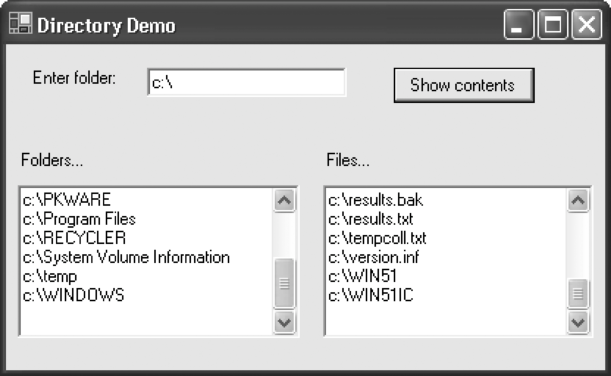
\includegraphics[width=12cm]{files_directory_screen}
			\caption{Screenshot of Directory Demo program.}
			\label{fig:files_directory_screen}
		\end{figure}
		
		First, some terminology. As you know, operating systems provide a hierarchical structure, with a path to a file of the form:
		\begin{lstlisting}
c:\data\exams.txt
		\end{lstlisting}
		This is a Windows-style path, with \textbackslash used as a separator. The terminology is that:
		\begin{itemize}
      \item the whole item is a path;
			\item the extension is \keyword{txt};
			\item the directory path is \keyword{c:\textbackslash data};
			\item the file name in the path is \keyword{exams.txt};
			\item if a program refers to a file without providing a directory (e.g. simply \keyword{exams.txt}), then the file is assumed to be in the same directory as the program is stored in and executed from.
		\end{itemize}
		Now we will provide details of some selected methods of the \keyword{Directory} class. They are shared: they provide useful methods for operating on strings that contain file paths.

		\subsection*{\keyword{GetFiles}}
			This method operates on a string containing a directory path. It returns an array of strings containing all the file names within the specified directory. The following program (Directory Demo) shows it in action.
			Sometimes we might need to check on the type of a file before opening it. Here is an example which checks if a file name ends in \keyword{.txt}. In Windows, capitals can also be used, so we convert the file name to upper-case before testing it. The \keyword{EndsWith} string method is convenient:
		\begin{lstlisting}
Dim fileName As String = "c:\tests\demo.txt"
If fileName.ToUpper().EndsWith(".TXT") Then
	MessageBox.Show("a text file")
End If
		\end{lstlisting}

		\subsection*{GetDirectories}
			This method operates on a string containing a directory name. It returns an array of strings containing the names of all the directories within the specified directory.
		\begin{lstlisting}
Dim dirs() As String = Directory.GetDirectories("c:\")
		\end{lstlisting}
		The following program shows it in action. Note that this method does not work through a directory tree to the very bottom. It only goes one level deep. Repeated calls of \keyword{GetFiles} are needed to progress deeper.
		
		Here is a program, named Directory Demo, with its screenshot in \Vref{fig:files_directory_screen} The user can enter a directory name, and the program displays the name of every file and every directory in the chosen directory.
		\begin{lstlisting}
Private Sub Button1_Click(sender As System.Object
			, e As System.EventArgs)
			Handles Button1.Click
	Dim files() As String =
			Directory.GetFiles(FileNameBox.Text)
	Dim count As Integer
	For count = 0 To UBound(files)
		FilesBox.AppendText(files(count) & NewLine)
	Next
	'display all directory names
	Dim dirs() As String =
			Directory.GetDirectories(FileNameBox.Text)
	For count = 0 To UBound(dirs)
		FolderBox.AppendText(dirs(count) & NewLine)
	Next
End Sub
		\end{lstlisting}
		Once we have filled our arrays, we can use the \keyword{UBound} function to control a loop which looks at each element in turn.

		
	\section{Programming principles}
		\begin{itemize}
      \item Programs use streams to read and write data to files.
      \item We use files to preserve data after the run of the program, or for passing data to other programs.
		\end{itemize}


	\section{Programming pitfalls}
		\begin{itemize}
      \item Forgetting to put any required importing details at the very top of the code. We used:
		\begin{lstlisting}
Imports System.IO
Imports Microsoft.VisualBasic.ControlChars
		\end{lstlisting}
		The latter provides us with \keyword{NewLine} for use in text boxes.
		\end{itemize}


	\section{Grammar spot}
		\begin{itemize}
      \item We declare and create file streams by, e.g.:
				\begin{lstlisting}
Dim inputStream As StreamReader =
	File.OpenText("c:\myfile.txt")
Dim outputStream As StreamWriter =
	File.CreateText("c:\myfile.txt")
				\end{lstlisting}
      \item We can read a file line-by-line with:
				\begin{lstlisting}
Dim line As String
line = inputStream.ReadLine()
While line <> Nothing
	' process the line . . .
	line = inputStream.ReadLine()
End While
		\end{lstlisting}
				or we can read the whole file at once with the \keyword{ReadToEnd} method.
      \item We close streams by, e.g.:
				\begin{lstlisting}
outStream.Close();
				\end{lstlisting}
		\end{itemize}


	\section{New language elements}
		We have introduced these classes:
		\begin{itemize}
			\item \keyword{File}
      \item \keyword{Directory}
      \item \keyword{StreamReader} and \keyword{StreamWriter}
      \item \keyword{FileNotFoundException}
      \item \keyword{SaveFileDialog} and \keyword{OpenFileDialog}
		\end{itemize}


	\section{New IDE facilities}
		\begin{itemize}
      \item We can place a main menu on a form, and handle menu item clicks via a method that VB generates.
      \item We can place file dialogs onto a form. (They move to the component tray.) We can manipulate their properties at design-time and run-time.
		\end{itemize}


	\section{Summary}
		\begin{itemize}
      \item Files are opened, then written to (or read from), and finally closed.
      \item The \keyword{Directory} class allows you to access the contents of a directory. Its methods allow you to access the names of its sub-directories and its files.
		\end{itemize}

	\section{Exercises}
		\begin{EXE}
			\item	Write a program which puts your name and address in a file named \keyword{address.txt}. Use an editor to check that the file has the expected contents.
			\item	Write a program to count the number of lines in a file. Ensure that it works for an empty file (producing a value of zero).
			\item	Write a program which examines each line of a file to see if it contains a particular string. Append each of those lines to a multiline text box, preceded by the file name. Use another text box to hold the string to search for.
			\item	Write a program which reads two files line-by-line, and compares them for equality. It should display a message stating that the files are either equal or not equal. Obtain the file names by displaying two file dialogs.
			\item	Write a program which replaces one string with another in each line of a file, writing the new version to another file. Use two text boxes for the 'from' and 'to' strings. You could use the \keyword{Change} method created in \Cref{ch:strings}.
			\item	This question involves writing two programs, which assist in extracting parts of files and inserting the parts into other files. For example, you might use them to insert code examples in an essay, or to insert standard headings at the start of a file.
				\begin{itemize}
		      \item Write a program which reads a file line-by-line, copying those lines between special markers to an output file. Here is an example of an input file:
						\begin{verbatim}
Though most blues guitar players
are right-handed, (or left-handed
players who re-strung their guitars,
such as Jimi Hendrix), two left-handed
players have made their mark:
EXTRACTTO:king.txt
Albert King, whose style involves
long bent notes, played slowly.
ENDEXTRACT
EXTRACTTO:rush.txt
Otis Rush, who is a highly-rated
songwriter and singer.
ENDEXTRACT
However, such an approach restricts
the player to simple chord fingerings.
						\end{verbatim}
						The lines between the first extract are to be copied to the file \keyword{king.txt}, and the second extract is to be copied to \keyword{rush.txt}.
    		  \item Write a program which copies one file line-by-line to another file. Any 'insert' instructions cause the specified file to be inserted in the input file. Here is an example:
						\begin{verbatim}
List Of Players:
INSERTFROM:king.txt
INSERTFROM:rush.txt
						\end{verbatim}
						Assume that the files are as above, with no errors in the use of the special insert/extract lines.
				\end{itemize}
			\item	Write a program which calculates the total number of lines stored in all the text files in a specified folder.
			\item	Write a program which examines each \keyword{txt} file in a selected folder for lines containing a particular string. Any such lines are to be appended to a multiline text box, preceded by their file name. Use a text box to allow the user to enter the string to find.
			\item	Write a program which appends the first 10 lines of every \keyword{.txt} file in a selected folder to a multiline text box, preceded by the file's name. If the file contains less than 10 lines, every line is to be displayed.
		\end{EXE}

		\begin{stab}
			\begin{enumChapter}
				\item	It creates a file containing the following text:
					\begin{verbatim}
*
**
***
	etc
					\end{verbatim}
					If we omitted to use \keyword{WriteLine}, all the stars would appear on one long line.
				\item	When \keyword{Nothing} is returned at the end of the file, its length is displayed, resulting in a value of zero. We need to reverse the order of the two statements within the loop, so that the use of \keyword{ReadLine} is immediately followed by going up to the start of the loop and the test for end-of-file.
				\item	The program loops forever (or at least until the text box becomes full), because there is no \keyword{ReadLine} in the middle of the loop.
				\item	We can convert each item to e.g. upper case, as in:
					\begin{lstlisting}
If Trim(words(0)).ToUpper() = studentName.Text.ToUpper() Then
	etc.
					\end{lstlisting}
				\item	A \keyword{While} loop repeats until the complete condition becomes false. Assume that we have two conditions that are initially true, with an \keyword{Or} between them. One condition becoming false does not make the whole condition false, because the other condition is still true.
					On the other hand, if we connect the two conditions with \keyword{And}, one condition changing to false makes the overall condition false. It is correct to use \keyword{And} in our search. In our incorrect \keyword{Or} example, if the data is not found, there is no way out of the loop, because both conditions can never become false. The program loops forever.
				\item	We provide a question-mark icon and yes/no buttons, as in:
					\begin{lstlisting}
If MessageBox.Show("Is Paris the capital of France?",
			"Quiz",
			MessageBoxButtons.YesNo,
			MessageBoxIcon.Question)
		= DialogResult.Yes Then
	MessageBox.Show("Yes – correct!")	
Else
	MessageBox.Show("Sorry... wrong.")
End If
					\end{lstlisting}
				\item We add this code to the save menu event:
					\begin{lstlisting}
If MessageBox.Show("Do you really want to save?",
			"Text Editor",
			MessageBoxButtons.YesNo,
			MessageBoxIcon.Question)
		= DialogResult.Yes Then
	MessageBox.Show("user clicked Yes")
	'code to save the text box in the file...
End If	
					\end{lstlisting}
			\end{enumChapter}
		\end{stab}

